\documentclass[]{scrartcl}
	
%opening
\title{Orbital Gravity Simulation}
\subtitle{An implementation of newtonian mechanics in Scala and OpenGL}
\author{Freddie Poser}
\date{2016}
\usepackage{hyperref} 
\usepackage{url}
\usepackage[hyphenbreaks]{breakurl}
\usepackage{xcolor}
\usepackage{listings}
\usepackage{graphicx}
\usepackage{wrapfig}
\usepackage{caption}
\usepackage[list=true]{subcaption}
\usepackage{import}

\graphicspath{ {img/} }
\lstset{
	basicstyle=\small\ttfamily,
	numbers=left,
	breaklines=true,
	postbreak=\raisebox{0ex}[0ex][0ex]{\ensuremath{\color{red}\hookrightarrow\space}},
	keywordstyle=\color{orange},
	stringstyle=\color{darkgreen},
	commentstyle=\color{gray},
	morecomment=[l][\color{magenta}]{\#}
}

\lstdefinelanguage{Scala}{	
	morekeywords={abstract,case,catch,class,def,
		do,else,extends,false,final,finally,
		for,if,implicit,import,match,mixin,
%		new,null,object,override,package, 
		private,protected,requires,return,sealed,
		super,this,trait,true,try,
		type,val,var,while,with,yield},
	sensitive,
	morecomment=[l]//,
	morecomment=[n]{/*}{*/},
	morestring=[b]",
	morestring=[b]',
	morestring=[b]""",
}
\lstset{language=Scala}
\begin{document}




\maketitle

\begin{abstract}
An implementation of Newtonian mechanics designed to simulate gravity and interactions between particles in two dimensions.
\end{abstract}

\tableofcontents
\listoffigures
\newpage

\section{Plan}
	The plan for this project is to simulate the motion of round particles in two dimensions. The particles will exert Newtonian gravity on each other and will be able to collide. This will all be implemented using Newtonian mechanics, namely Newton's second law and the kinematic laws of motion.
	
	For the motion I will assume that acceleration is constant for 1 second and so the simulation will update in steps, each representing 1s. It may be possible in the future to decrease this for more accurate simulations (or increase it for faster ones).
	
	I am going to build this in with Scala, a JVM programming language. The advantage of Scala is that it is multi-paradigm, allowing me to use OOP and functional programming concepts. For the graphics I will use an OpenGL wrapper library called LWJGL\footnote{\url{https://www.lwjgl.org/}}.
	
	Using this will allow me to watch the simulation in real-time rather than look at the data it outputs after the fact. I may implement a way of getting the raw data out of the simulation as well so that I can simulate real situations with greater ease.
	
	Below is an overview of the features that I implemented in the program. They are covered in the order that I implemented them.
\newpage
\section{Setup}
	
	\sloppy
	All of the source code is available at \burl{https://github.com/vogon101/NewtonianMechanics}
	
	Below is a list of a few of the core classes in the simulation
	
	\subsection{Universe}
		\fussy	
		The Universe class manages the overall simulation. The key part of Universe is its list of all the particles in existence. The Universe also contains the GraphicsManager which controls all of the rendering and adds a layer of abstraction between the simulation and the OpenGL bindings. 
		
	\subsection{Particle}
		
		The Particle class represents every single object in the system. The particles all have a ParticleType which defines their intrinsic properties: radius, mass, colour as well as a position vector. Each particle is able to render itself which involves drawing the appropriate circle at its location, the path that it has been on and all of the forces acting on it.
		\linebreak\linebreak
		The key physics is contained in the methods interact(that: Particle) and runTick():
		
		\subparagraph{interact}
		
			Interact is called by the universe class before every tick is run. For every unique pair of particles in system interact is called once. It takes in the particle to interact with and returns a list of forces generated by the interaction.
			
			These forces are then taken by the universe class and applied to their target particles, storing them up for the next time runTick is called.
		
		\subparagraph{runTick}
			
			RunTick is called on every particle each time the simulation updates after all of the interactions are computed. It returns no value but instead computes the effects of the forces and updates the particles position and velocity accordingly.
			
			The effective input to runTick is a list of forces and it then performs the following calculations (t = length of tick in this case):
			
			\begin{figure}
				\begin{equation}
					\vec{F_{R}} = \vec{F_{1}} + \vec{F_{2}} ... \vec{F_{n}}
				\end{equation}
				
				\begin{equation}
					\vec{a} = \frac{\vec{F_{R}}}{m}
				\end{equation}
				
				\begin{equation}
					\vec{v} = \vec{u} + \vec{a}t
				\end{equation}
				
				\begin{equation}
					\vec{r} = \vec{r} + \vec{v}t
				\end{equation}
				\caption{Movement equations used in Particle class}
				\label{fig:movEqn}
			\end{figure}
		
			These equations are based first on Newton's second law of motion which gives that the net force on an object is equal to its mass times its acceleration ($\vec{F_{R}} = m\vec{a}$). With the acceleration I find the new velocity by multiplying it by the time it acts for and adding it to the old velocity. This model assumes constant acceleration and velocity for the duration of each tick. This means that the accuracy of the model is linked to the length of the tick, with the shorter they are, the better the simulation. The position is then found by applying the velocity in the same way.
	\newpage
	\subsection{Rendering}
		
		Rendering uses code that I originally wrote for a simple game engine (\href{https://github.com/vogon101/CottonGame}{Cotton Game})\footnote{\url{https://github.com/vogon101/CottonGame}}. This code does a number of things:
		
		\subparagraph{GraphicsManager} 
			
			The graphics manager class controls the basic screen setup and the standard OpenGL commands that need to be called to simply get rendering working.
		
		\subparagraph{Sync} 
		
			The sync class is a utility that allows the programmer to control how often a given method is run in a non-blocking fashion. In this project it is used in three places:
			
			\begin{itemize}
			\item Render Sync - locks the render loop at 60FPS
			
			\item Update Sync - allows the user to choose how fast to run the simulation
			
			\item UX Sync - separates the input polling from the update sync so that even if the game is paused the user can still control it
		\end{itemize}
		
		\subparagraph{Render} 
		
			The Render object is a static collection of utilities that make rendering easier to work with, they abstract away from the details of OpenGL so that code is cleaner and easier to debug
	
\newpage
	\section{Gravity}
	For gravity I use the Newtonian equation which provides the magnitude of the force between two bodies. I calculate this during the interact function so the force is calculated between every pair of particles in the universe.
	\begin{figure}[h]
		\begin{equation}
		F = G\frac{m_{1}m_{2}}{r^{2}}
		\end{equation}
		\caption{Newton's law of Universal Gravitation}
		\label{fig:gravEqn}
	\end{figure}\footnote{Source: \url{https://en.wikipedia.org/wiki/Newton's_law_of_universal_gravitation}}
	
	Once I have the magnitude I find its direction by finding the angle between the two position vectors and it is applied to each body.
	\begin{figure}[h]
		\centering
		\begin{lstlisting}[language=Scala]
val distance = that.position.distance(position)
val gravForce = (GRAVITATIONAL_CONSTANT * mass * that.mass) / Math.pow(distance, 2)

//Final forces from gravity
List(
  Force(that, gravForce, (this.position - that.position).theta),
  Force(this, gravForce, (that.position - this.position).theta)
)
		\end{lstlisting}
		\caption{The gravity calculations from the Particle class}
		\label{fig:gravCode}
	\end{figure}

	This creates two vector forces, one on each object which are used during the run tick phase.
	
	Whilst Newtonian gravity has been superseded by general relativity it is still a good approximation in almost all situations where great precision is not required and where the bodies move at low speeds. I have used it in this project because it is much easier to implement\footnote{\url{https://en.wikipedia.org/wiki/Newton's_law_of_universal_gravitation\#Problematic_aspects}}
	
	\begin{figure}[p]
		\centering
		\begin{subfigure}{0.9\textwidth}
			\centering
			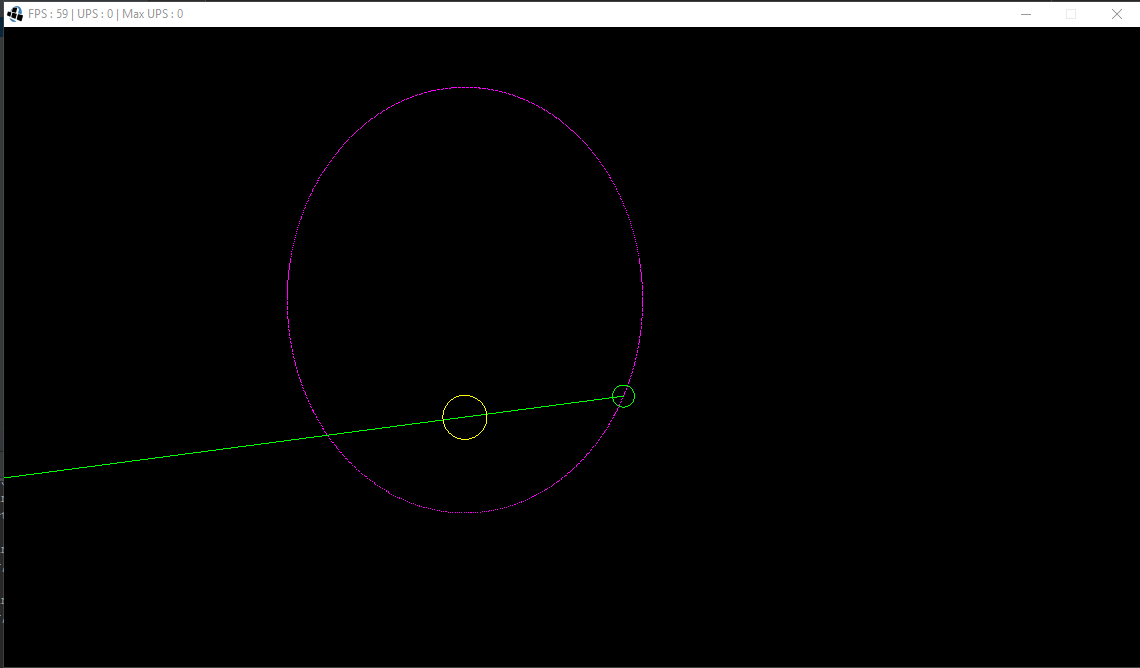
\includegraphics[width=\textwidth]{gravity1}
			\caption{One body in orbit, the orbit is perfectly stable in this case. The green line is the force on the planet.}
			\label{fig:gravExamplesSub1}
			\ref{fig:gravExamplesSub1}
		\end{subfigure}
		\begin{subfigure}{0.9\textwidth}
			\centering
			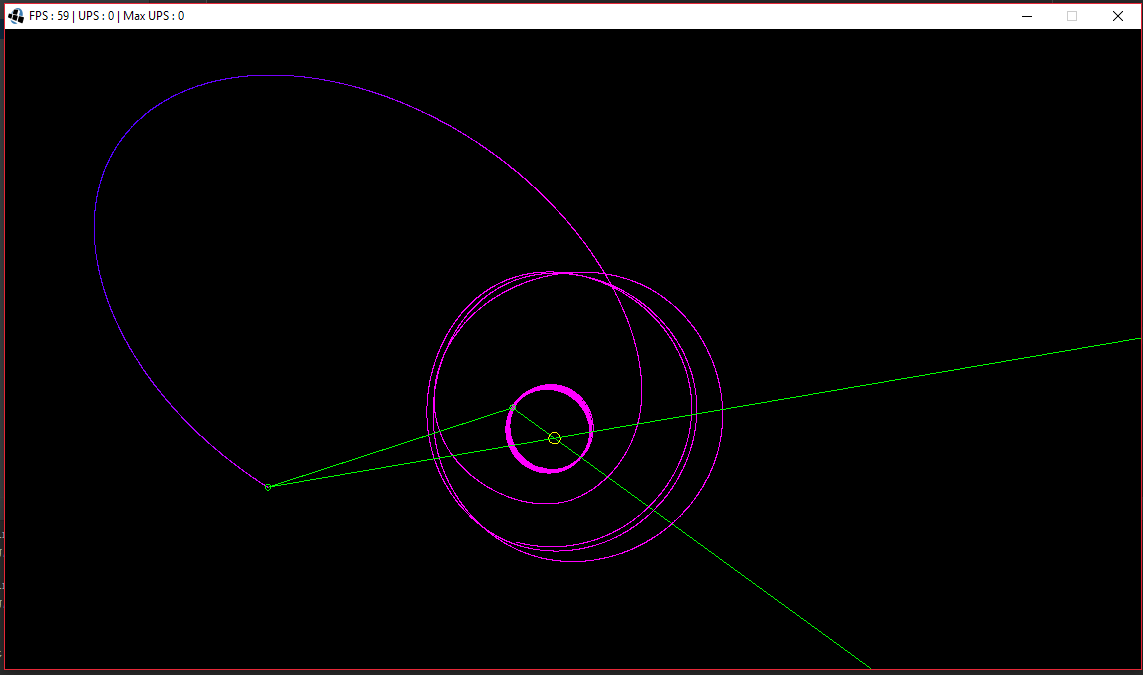
\includegraphics[width=\textwidth]{gravity2}
			\caption{Two bodies in orbit, one is on a more stable orbit whilst the outer one moves more erratically} 
			\label{fig:gravExamplesSub2}
			\ref{fig:gravExamplesSub2}
		\end{subfigure}	
		\caption{Examples of gravity with one and two bodies in orbit around a fixed star}
		\label{fig:gravExamples}
	\end{figure}
\newpage
\section{Momentum  and Collisions}
	Once I had implemented gravity I decided to add in simple 2D collisions to make the simulation slightly more realistic.
\newpage
\section{User Control}
	
	Whilst the majority of this project is the physics, I think it is important that it is possible to interact with the simulation to be able to watch it more effectively. To this end I have built a command system which allows the user to control parts of the simulation along with certain key bindings.
	
	\begin{figure}[h]
		\begin{itemize}
			\item \textbf{+}/\textbf{-} $\rightarrow$ Speed up/slow down the simulation
			\item \textbf{LSHIFT} + \textbf{+}/\textbf{-} $\rightarrow$ Zoom in/out
			\item \textbf{LEFT}/\textbf{RIGHT} $\rightarrow$ Pan around the simulation horizontally
			\item \textbf{UP}/\textbf{DOWN} $\rightarrow$ Pan around the simulation vertically
		\end{itemize}
		\caption{Key bindings for the simulation}
		\label{fig:keybindings}
	\end{figure}
	
	\begin{figure}[h]
		\begin{itemize}
			\item track $<$particle num$>$ $\rightarrow$ Track a certain particle
			\item cleartrack $\rightarrow$ Clear the tracker, allow free movement
			\item show $\rightarrow$ Print a list of particles to STD Out
			\item forces $\rightarrow$ Toggle rendering of forces
			\item col $<$on/off$>$ $\rightarrow$ Render collision forces even if force rendering disabled
			\item particle $<$particle num$>$ $\rightarrow$ Centre view on a particle
			\item pause $\rightarrow$ Pause the simulation
			\item slow $\rightarrow$ Slow down the simulation to 10 UPS
			\item 1 $\rightarrow$ Set the maximum UPS to 1 (real time)
			\item speed $<$UPS$>$ $\rightarrow$ Set the speed of the simulation (sets max UPS)
			
			
		\end{itemize}
		\caption{Commands for the simulation}
		\label{fig:commands}
	\end{figure}
	
	\begin{figure}
		\centering
		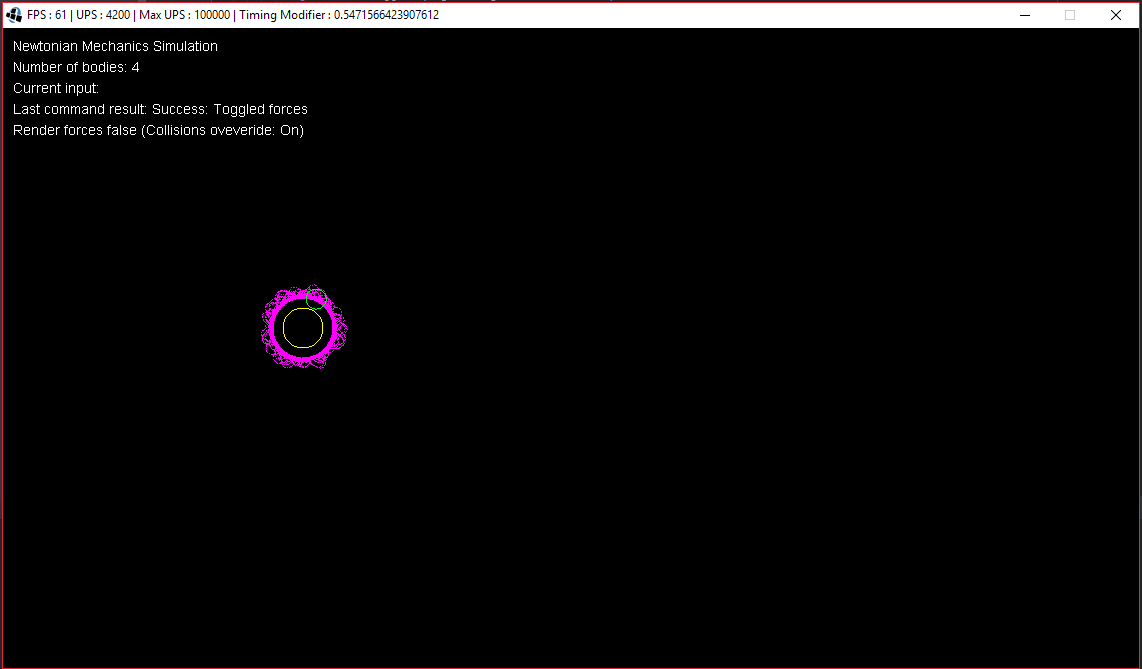
\includegraphics[width=\textwidth]{ux1}
		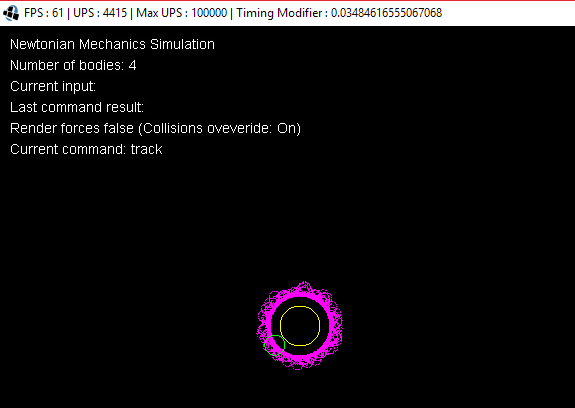
\includegraphics[width=\textwidth]{ux2}
		\caption{Information about the simulation displayed in the top left corner}
		\label{fig:uxImg1}
	\end{figure}
	
	

\end{document}
